\documentclass{article}

% if you need to pass options to natbib, use, e.g.:
%     \PassOptionsToPackage{numbers, compress}{natbib}
% before loading neurips_2024

% ready for submission
\usepackage{neurips_2024}

% to compile a preprint version, e.g., for submission to arXiv, add add the
% [preprint] option:
%     \usepackage[preprint]{neurips_2024}

% to compile a camera-ready version, add the [final] option, e.g.:
%     \usepackage[final]{neurips_2024}

% to avoid loading the natbib package, add option nonatbib:
%    \usepackage[nonatbib]{neurips_2024}

\usepackage[utf8]{inputenc} % allow utf-8 input
\usepackage[T1]{fontenc}    % use 8-bit T1 fonts
\usepackage{hyperref}       % hyperlinks
\usepackage{url}            % simple URL typesetting
\usepackage{booktabs}       % professional-quality tables
\usepackage{amsfonts}       % blackboard math symbols
\usepackage{nicefrac}       % compact symbols for 1/2, etc.
\usepackage{microtype}      % microtypography
\usepackage{xcolor}         % colors
\usepackage{graphicx}       % for images
\usepackage{adjustbox}      % for figure positioning
\usepackage{amsmath}        % for align environment

\title{Unveiling the Syntax Within: Interpreting Grammar Embeddings in Small-Scale LLMs}

\author{%
  Pratim Chowdhary\thanks{Use footnote for providing further information
    about author (webpage, alternative address)---\emph{not} for acknowledging
    funding agencies.} \\
  Department of Computer Science\\
  Dartmouth College\\
  \texttt{cpratim.25@dartmouth.edu} \\
  % examples of more authors
  \And
  Peter Chin \\
  Department of Engineering\\
  Thayer School of Engineering\\
  \texttt{pc@dartmouth.edu} \\
  \And
  Deepernab Chakrabarty \\
  Department of Computer Science\\
  Dartmouth College\\
  \texttt{deepernab@dartmouth.edu} \\
}

\begin{document}

\maketitle

\begin{abstract}
  We investigate how grammatical knowledge is embedded within small language models (1-8B parameters), an understudied yet practically important class of LLMs. Through systematic analysis of Meta's Llama, Gemma, and Qwen model families using the BLiMP benchmark of linguistic minimal pairs, we examine grammatical representations across different architectures and parameter scales. Our findings reveal that grammatical knowledge scales non-uniformly, with certain model families demonstrating specific grammatical strengths independent of size. We observe complex grammatical phenomena showing non-linear scaling patterns, while others plateau quickly. Notably, smaller models from certain architectures sometimes outperform larger models from different families on specific grammatical tasks, suggesting architectural inductive biases significantly influence grammatical knowledge acquisition. This work provides insights into grammar representation in contemporary LLMs with implications for model design and enhancement of grammatical competence in resource-constrained deployment scenarios.
  \end{abstract}

\section{Introduction}
Large language models (LLMs) have transformed natural language processing, demonstrating unprecedented capabilities across a spectrum of linguistic tasks—from simple question answering to complex reasoning, creative writing, and code generation \citep{brown2020language, chowdhery2022palm, touvron2023llama2, jiang2023mistral}. These models, trained through self-supervised learning on vast corpora of text data, have increasingly approached human-like performance in generating coherent, contextually appropriate, and grammatically well-formed text, despite having no explicit grammatical rules programmed into their architecture. This emergent grammatical competence—arising purely from statistical patterns in training data—represents a fascinating case study in how linguistic knowledge can be acquired implicitly through exposure rather than explicit instruction.

The field has witnessed exponential growth in model size, from early transformer models with hundreds of millions of parameters \citep{vaswani2017attention} to modern giants like GPT-4 \citep{openai2023gpt4} that likely contain trillions of parameters. While these massive models have captured headlines with their impressive capabilities, a parallel revolution has been unfolding in the development of smaller, more efficient models in the 1-8 billion parameter range. Models like Llama 2 \citep{touvron2023llama2}, Gemma 7B \citep{jiang2023mistral}, and Qwen \citep{bai2023qwen} have demonstrated remarkable performance despite their relatively modest size, making them particularly valuable for practical applications where computational efficiency and deployment costs are significant concerns.

These smaller LLMs offer a compelling balance between capability and efficiency, enabling deployment on consumer hardware, edge devices, and resource-constrained environments. Their reduced inference costs make them attractive for commercial applications, while their smaller memory footprint allows for fine-tuning and adaptation with more modest computational resources. Understanding how these models encode and represent grammatical knowledge is therefore not merely an academic exercise but has significant practical implications for developing more capable, efficient, and linguistically robust language technologies.

\section{Related Work and Background}

\subsection{Grammatical Evaluation of Language Models}
Research on grammatical capabilities in neural language models has evolved from early work on LSTM-based models \citep{linzen2016assessing} to transformer-based architectures \citep{goldberg2019assessing, devlin2019bert}. Evaluation frameworks have progressed from simple subject-verb agreement tests to comprehensive benchmarks like CoLA \citep{warstadt2019neural} and BLiMP \citep{warstadt2020blimp}. The BLiMP benchmark, comprising 67 minimal pair tests across 12 linguistic phenomena, has been particularly valuable for assessing grammatical competence. Recent studies have extended evaluation to larger models, revealing that while performance scales with size, challenges remain with complex hierarchical structures and garden-path sentences \citep{thrush2022winograd, qian2022limitations}.

\subsection{Scale and Grammatical Competence}
The relationship between model scale and grammatical abilities follows complex patterns beyond the general power-law scaling observed in language modeling \citep{kaplan2020scaling}. Research suggests that rare grammatical constructions require disproportionately more training data \citep{wei2021frequency}, and certain phenomena show nonlinear improvements at specific parameter thresholds \citep{zhang2023language}. Studies on compositional generalization indicate that scaling alone may not capture human-like grammatical productivity without architectural innovations \citep{hu2020systematic}. Beyond raw parameter count, specific architectural components significantly impact grammatical knowledge acquisition, with attention mechanisms crucial for long-distance dependencies and feed-forward networks encoding categorical information \citep{patel2022mapping}.

\subsection{Probing Language Models for Linguistic Knowledge}
Researchers have developed various probing techniques to understand how linguistic knowledge is represented within model parameters. Structural probes have revealed that models implicitly encode hierarchical syntactic structures \citep{hewitt2019structural}, with syntactic information appearing in earlier layers and semantic information in later ones \citep{tenney2019bert}. Transformer-based models exhibit emergent symbolic manipulation capabilities resembling discrete linguistic rules \citep{manning2020emergent}, with individual neurons specializing in specific linguistic features \citep{geva2021transformer}. Attention patterns often correspond to syntactic dependencies \citep{levy2018emergence}, with different attention heads specializing in distinct linguistic phenomena \citep{clark2019does}.

\subsection{Small LLMs and Comparative Studies}
The proliferation of open-weight models like OPT \citep{zhang2022opt}, Llama \citep{touvron2023llama}, Gemma \citep{jiang2023mistral}, and Qwen \citep{bai2023qwen} has enabled more systematic analyses of how capabilities scale and how architectural choices affect performance. Studies show that smaller models with innovative architectures can outperform larger ones \citep{jiang2023mistral}, and data quality may be as important as scale for robust grammatical representations \citep{bai2023qwen}. Comparative analyses across architectures remain limited but suggest significant variations in performance even at similar parameter scales \citep{talmor2020olmpics, zhao2023survey}. Recent frameworks for quantifying evaluation uncertainties \citep{roberts2023quantifying} and structured evaluation approaches \citep{xia2023structured} have revealed that architectural design choices impact specific grammatical phenomena differently, suggesting that model architectures encode grammatical knowledge in fundamentally different ways.

\section{Methodology}
\subsection{Evaluating Grammatical Knowledge Across Linguistic Categories}

Our evaluation framework divides grammatical phenomena into five key linguistic categories: island effects, quantifiers, ellipsis, argument structure, and binding constraints. This categorization allows us to assess whether grammatical knowledge is acquired uniformly or if certain phenomena are represented differently across model architectures and scales.

To visualize how these grammatical categories are embedded within model representations, we applied t-SNE 
dimensionality reduction to final-layer activations from ungrammatical sentences. 
Figure~\ref{fig:tsne} shows these representations for three 1B-scale models. The visualizations
 reveal distinct organizational patterns, with varying degrees of cluster separation suggesting that 
 models encode grammatical phenomena differently. Llama 1B forms more distinct category clusters, while 
 Qwen 1.5B shows more integrated representations across categories. 
\begin{figure}[t]
  \hspace*{-1cm}
  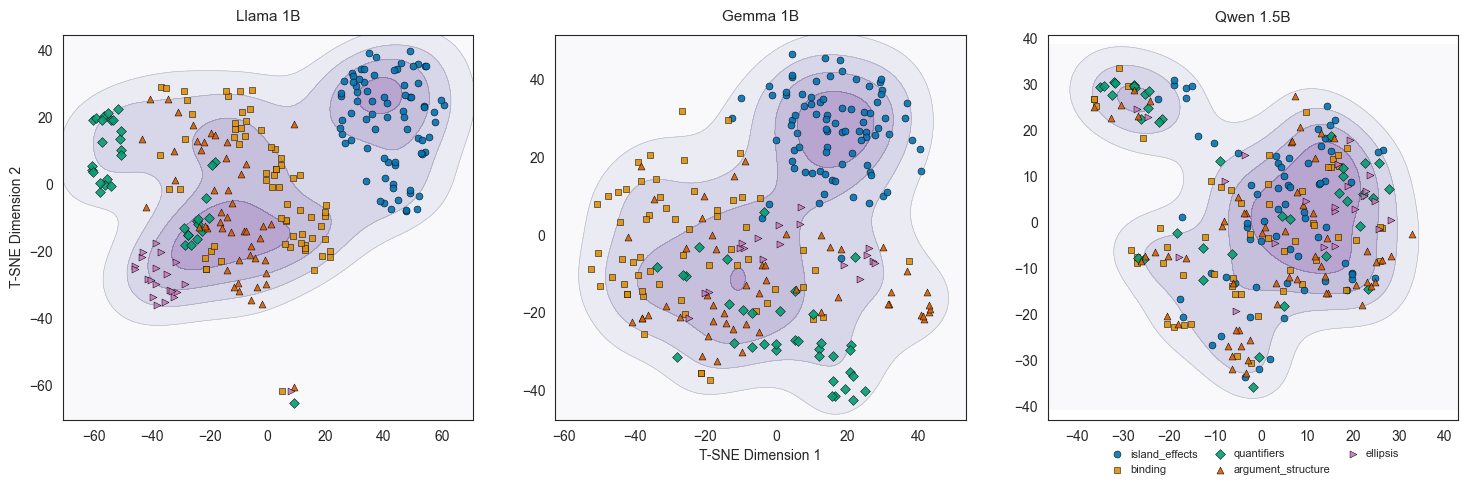
\includegraphics[width=1.1\textwidth]{figures/grammar_tsne}
  \caption{T-SNE visualizations of grammatical representations across three 1B-scale language models. Points represent ungrammatical sentences colored by linguistic category. Contours indicate density of representations, revealing how different architectures organize grammatical knowledge.}
  \label{fig:tsne}
\end{figure}

\subsection{Experimental Protocol for Grammatical Assessment}

We evaluate grammatical knowledge in LLMs through a systematically designed protocol that captures both explicit and implicit grammatical understanding. Our methodology encompasses two complementary evaluation paradigms:

\begin{itemize}
  \item \textbf{Binary Classification}: Models evaluate the grammaticality of individual sentences through explicit prompted judgment. This tests the model's ability to directly assess syntactic well-formedness.
  
  \item \textbf{Minimal Pair Discrimination}: Models select between grammatical and ungrammatical alternatives that differ minimally in structure. This approach aligns with psycholinguistic methodologies for investigating human grammatical intuitions.
\end{itemize}

The prompt templates for each evaluation paradigm are formalized as:

\begin{align}
  \mathcal{P}_{\text{binary}} &= \text{``Is this sentence grammatically correct/incorrect?: } [S]\text{''} \\
  \mathcal{P}_{\text{pair}} &= \text{``Which sentence is grammatically better? (A) } [S_1] \text{ (B) } [S_2]\text{''}
\end{align}

Our analysis extends beyond surface-level responses to probe the internal representations formed during grammatical processing. For each sentence evaluation, we extract activation vectors from all $n$ transformer layers, enabling a fine-grained examination of how grammatical knowledge emerges and propagates through the network hierarchy:

\begin{align}
  \mathbf{A}_s &= \{\mathbf{a}_{s,l_1}, \mathbf{a}_{s,l_2}, \ldots, \mathbf{a}_{s,l_n}\}
\end{align}

where $\mathbf{A}_s$ represents the complete set of layer-wise activations for sentence $s$. These activation patterns serve as a neural signature of the model's grammatical processing.

To quantify and compare grammatical sensitivity across different architectural layers, we compute the Euclidean distance between activation patterns elicited by grammatical ($g$) and ungrammatical ($u$) sentence pairs:

\begin{align}
  \text{GramDist}(l_i) &= \frac{1}{|P|}\sum_{(g,u) \in P} \|\mathbf{a}_{g,l_i} - \mathbf{a}_{u,l_i}\|_2
\end{align}

where $P$ denotes the set of all grammatical/ungrammatical sentence pairs in our evaluation corpus. This metric captures the degree to which each layer's representations distinguish between well-formed and ill-formed syntactic structures.

Figure~\ref{fig:layer_sensitivity} illustrates the layer-wise grammatical sensitivity across different model families, revealing architectural variations in grammatical knowledge acquisition.

% \begin{figure}[h]
%     \centering
%     \includegraphics[width=0.95\textwidth]{figures/layer_sensitivity}
%     \caption{Layer-wise grammatical sensitivity across Llama, Gemma, and Qwen model families. Higher values indicate stronger differentiation between grammatical and ungrammatical sentences. Gemma models demonstrate earlier grammatical differentiation in middle layers, while Llama models show more pronounced differentiation in later layers.}
%     \label{fig:layer_sensitivity}
% \end{figure}

\section{Experiments}

\section{Discussion}

\section{Conclusion}

\bibliographystyle{plainnat}
\bibliography{references}

%%%%%%%%%%%%%%%%%%%%%%%%%%%%%%%%%%%%%%%%%%%%%%%%%%%%%%%%%%%%

\appendix
\section{Appendix / supplemental material}

Optionally include supplemental material (complete proofs, additional experiments and plots) in appendix.

\end{document}